\documentclass{article}

% if you need to pass options to natbib, use, e.g.:
% \PassOptionsToPackage{numbers, compress}{natbib}
% before loading nips_2016
%
% to avoid loading the natbib package, add option nonatbib:
% \usepackage[nonatbib]{nips_2016}

%\usepackage{nips_2016}

% to compile a camera-ready version, add the [final] option, e.g.:
\usepackage[final]{nips_2016}

\usepackage[utf8]{inputenc} % allow utf-8 input
\usepackage[T1]{fontenc}    % use 8-bit T1 fonts
\usepackage{hyperref}       % hyperlinks
\usepackage{url}            % simple URL typesetting
\usepackage{booktabs}       % professional-quality tables
\usepackage{amsfonts}       % blackboard math symbols
\usepackage{nicefrac}       % compact symbols for 1/2, etc.
\usepackage{microtype}      % microtypography

\usepackage{enumitem}
\usepackage{listings}
\usepackage{caption}
\usepackage{subcaption}
\usepackage{graphicx}
\usepackage{wrapfig}

\lstset{
  basicstyle=\small\ttfamily,
  frame=tb,
  numbers=left,
  numberstyle=\tiny,
  emph={%  
    val, for%
    },emphstyle={\bfseries}%  
}

\title{Samsara: Declarative Machine Learning\\ on Distributed Dataflow Systems}

% The \author macro works with any number of authors. There are two
% commands used to separate the names and addresses of multiple
% authors: \And and \AND.
%
% Using \And between authors leaves it to LaTeX to determine where to
% break the lines. Using \AND forces a line break at that point. So,
% if LaTeX puts 3 of 4 authors names on the first line, and the last
% on the second line, try using \AND instead of \And before the third
% author name.

\author{
  Author~A\\
  \texttt{authorA@email.com} \\
  \And
  Author~B\\
  \texttt{authorB@email.com} \\
}

\begin{document}
% \nipsfinalcopy is no longer used

\maketitle

\begin{abstract}
  The abstract.
\end{abstract}

\section{Introduction}

\begin{itemize}[noitemsep]
  \item data processing and ML on large datasets stored in distributed filesystems becoming ubiquitous, distributed dataflow systems such as Apache Spark~\cite{Zaharia2012} and Apache Flink~\cite{Alexandrov2014} hard to program without detailed understanding of underlying execution model. Usually require programs to be structured using second-order functions + UDF on partitioned datasets.
  \item highly non-declarative programming, stark contrast to common like R, MATLAB or numpy
\end{itemize}

\begin{itemize}[noitemsep]  
  \item Samsara is an easy-to-use domain specific language (DSL) for distributed large-scale machine learning on systems like Apache Spark and Apache Flink
  \item part of the Apache Mahout project
  \item uses Scala as programming/scripting environment
  \item system-agnostic, R-like DSL
  \item algebraic expression optimizer for distributed linear algebra, provides a translation layer to distributed engines
\end{itemize}

\section{Overview}

\subsection{Architecture}


Explain Figure~\ref{fig:architecture}, different layers, optimizer, logical + physical operators, different backends

\begin{figure}
  \centering
  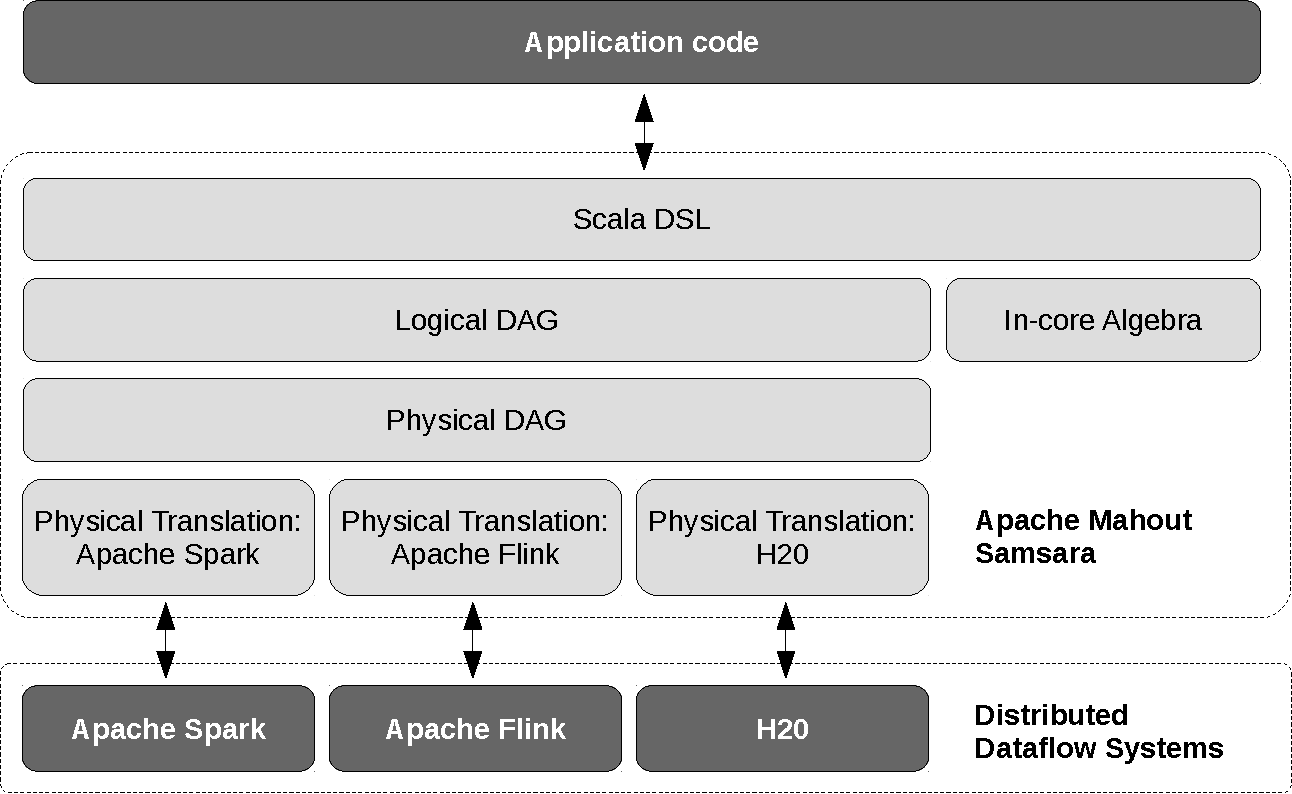
\includegraphics[scale=.5]{figures/architecture-crop}
  \caption{Architecture.}
  \label{fig:architecture}
\end{figure}

\subsection{Language Constructs}

Scalar real values; In-memory vectors: dense, 2 types of sparse; In-memory matrices, sparse and dense, a number of specialized matrices

Distributed Row Matrices (DRM)
huge matrix, partitioned by rows
lives in the main memory of the cluster
provides small set of parallelized 
       operations
lazily evaluated operation execution

matrix, vector, scalar operators: 
in-memory, distributed


slicing operators



assignments (in-memory only)


vector-specific

summaries

solving linear systems

in-memory decompositions



distributed decompositions; caching of DRMs

\subsection{Example: Distributed Ridge Regression}

Our running example throughout this paper will be the common task of predicting a continuous target vector $y$ from a feature matrix $X$ by ridge regression. For our example, we assume that $X$ is a tall and skinny matrix. We aim to compute the parameter vector $\beta$ of the regression by solving the normal equation: $\hat{\beta} = (X^\mathrm{T}X + \lambda I)^{-1} X^\mathrm{T}y$. In our implementation, we exploit the fact that $X^\mathrm{T} X$ as well as $X^\mathrm{T} y$ live in the column space of $X$ with small dimensionality (as $X$ is tall and skinny). This allows us to fit $X^\mathrm{T} X$ into memory of driver for moderate number of columns, as it will only require memory quadratic in the number of columns of~$X$.

The resulting Samsara program is shown in Listing~\ref{lst:linearRegression}. The code defines a function \texttt{dridge} which takes two arguments: a distributed data matrix containing the features and the target variable (in the right-most column), as well as the regularization parameter $\lambda$ (cf.,~line~1). We form the feature matrix $X$ by slicing out all columns except for the right-most one from the input data matrix, and append a column of ones for the bias term~(cf.,~line~2). Next, we slice out the right-post column of the input data matrix to retrieve the target vector~$y$~(cf.,~line~3). We compute $X^\mathrm{T} X$ via distributed matrix multiplication~(cf.,~line~5), and $X^\mathrm{T}y$ via distributed matrix vector multiplication~(cf.,~line~6). Finally, we materialize $X^\mathrm{T} X$  and $X^\mathrm{T} y$ on the driver (cf., the \texttt{collect} calls in~lines~8~\&~9), add the regularization term to the diagonal of $X^\mathrm{T} X$~(cf.,~line~11), and use an in-core solver to compute the parameter estimate $\beta$~(cf.,~line~13).

\begin{lstlisting}[caption={Distributed Ridge Regression for tall \& skinny matrices using Samsara.}\label{lst:linearRegression},captionpos=b] 
def dridge(data: DrmLike[Int], lambda: Double): Vector = {
  val drmX = data(::, 0 until data.ncol) cbind 1
  val y = data.collect(::, data.ncol)

  val drmXtX = drmX.t %*% drmX
  val drmXty = drmX.t %*% y

  val XtX = drmXtX.collect 
  val Xty = drmXty.collect(::, 0) 

  XtX.diagv += lambda

  solve(XtX, Xty)
}
\end{lstlisting}

\begin{figure}
    \centering
         \begin{subfigure}[b]{0.5\textwidth}
            \centering
            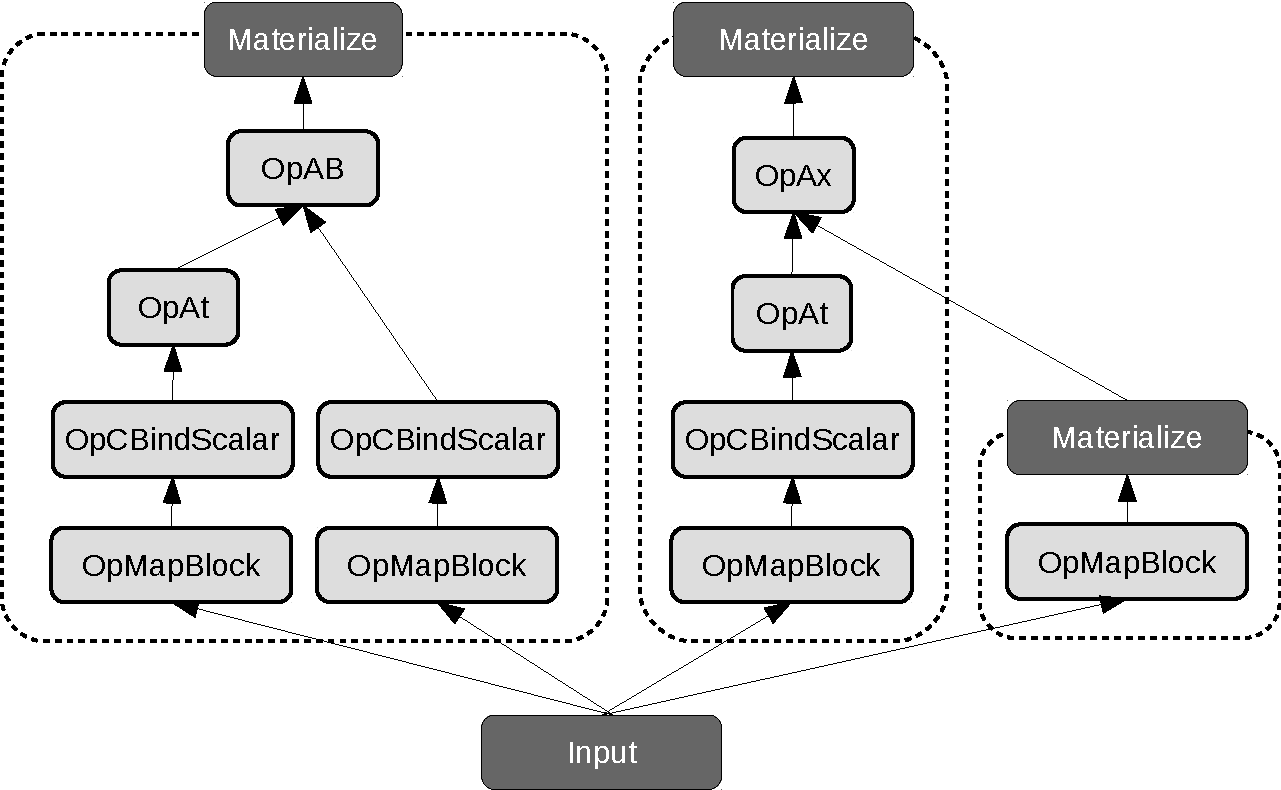
\includegraphics[scale=.33]{figures/linear-regression-logicalplan-crop}
            \caption{TBD.}
            \label{fig:logicalplan}
        \end{subfigure}
  \hfill
         \begin{subfigure}[b]{0.4\textwidth}
            \centering
            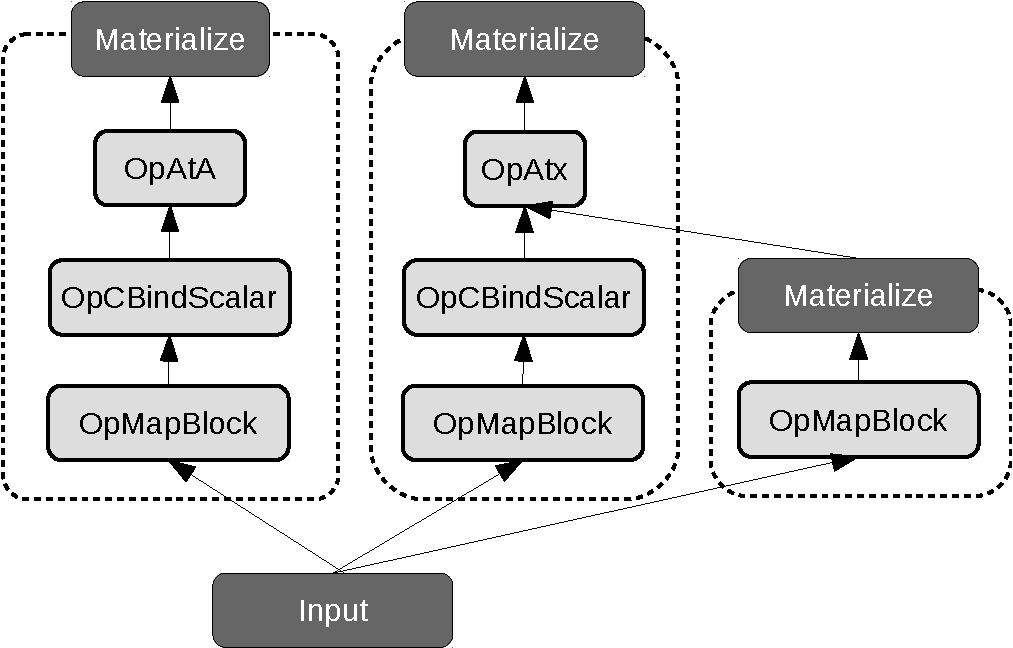
\includegraphics[scale=.33]{figures/linear-regression-logicalplan-optimized-crop}
            \caption{TBD.}
            \label{fig:logicalplan-optimized}
        \end{subfigure}
        \caption{\label{fig:logicalplans} Logical execution plan resulting from the distributed linear regression code in~Listing~\ref{lst:linearRegression} (before and after optimization).}
\end{figure}


\subsection{Runtime \& Optimization}

Execution is defered, user composes logical operators; Computational actions implicitly trigger optimization (= selection of physical plan) and execution; Optimization factors:  size of operands, orientation of operands, partitioning, sharing of computational paths; e. g.: matrix multiplication: 5 physical operators for drmA \%*\% drmB; 2 operators for drmA \%*\% inMemA; 1 operator for drm A \%*\% x; 1 operator for x \%*\% drmA; Computation of ATA in example; Naïve execution: 1st  pass: transpose A; (requires repartitioning of A); 2nd pass: multiply result with A; (expensive, potentially requires repartitioning again); Logical optimization: Optimizer rewrites plan to use; 

TODO explain Figure~\ref{fig:logicalplan}

Two-phase optimization, logical and physical. Optimization per DAG associated with a pipeline (all the operators between two materializations).

\subsubsection{Logical Optimization}

In the logical optimization phase, Samsara uses pattern matching to derive rewritten plans that still produce same result, but potentially with less runtime. Samsara's optimizer is rule-based and its rewrites aim at reducing the number of passes over the input data, typically plan is compacted by merging operators. 

Figure~\ref{fig:logicalplan-optimized} shows the final plan to execute produced by optimizing the original plan for our example code from Figure~\ref{fig:logicalplan}. The expression \texttt{OpAt $\rightarrow$ OpAx} which represents the computation of $X^\mathrm{T}y$ from the middle pipeline in~Figure~\ref{fig:logicalplan} is merged into the operator \texttt{OpAtx} in the optimized plan illustrated in Figure~\ref{fig:logicalplan-optimized}. The latter operator is a specialed implementation to compute a matrix transpose times vector multiplication in a single pass over the input. The next expression that gets optimized is \texttt{OpMapBlock $\rightarrow$ OpCbindScalar $\rightarrow$ OpAt $\rightarrow$ OpAB $\leftarrow$ OpCbindScalar $\leftarrow$ OpMapBlock}. This expression represents the part of the code that slices out $X$ from the input matrix and subsequently computes $X^\mathrm{T}X$. This expression is rewritten in two steps: first, the partial expression \texttt{OpAt $\rightarrow$ OpAB} is merged to \texttt{OpAtB}, so that the full expression becomes \texttt{OpMapBlock $\rightarrow$ OpCbindScalar $\rightarrow$ OpAtB $\leftarrow$ OpCbindScalar $\leftarrow$ OpMapBlock}. Second, we recognize that both of the inputs to \texttt{OpAtB} refer to same matrix, which allows us to replace \texttt{OpAtB} with a special operator \texttt{OpAtA} for transpose-times-self matrix multiplications. This saves us from having to compute the result of \texttt{OpMapBlock $\rightarrow$ OpCbindScalar $\rightarrow$ OpAt}, and shrinks the resulting DAG down to \texttt{OpMapBlock $\rightarrow$ OpCbindScalar $\rightarrow$ OpAtA}.

\subsubsection{Physical Optimization}

Two physical operators (concrete implementations) available for Transpose-Times-Self operation: standard operator AtA; operator AtA\_slim, specialized implementation for tall \& skinny matrices; Optimizer must choose; currently: depends on user-defined threshold for number of columns; ideally: cost based decision, dependent on estimates of intermediate result sizes; specialized logical operator for Transpose-Times-Self matrix multiplication; Samsara computes ATA via row-outer-product formulation; executes in a single pass over row-partitioned A~\cite{Schelter2012}; 

\begin{figure}[b]
    \centering
         \begin{subfigure}[b]{0.45\textwidth}
  \centering
  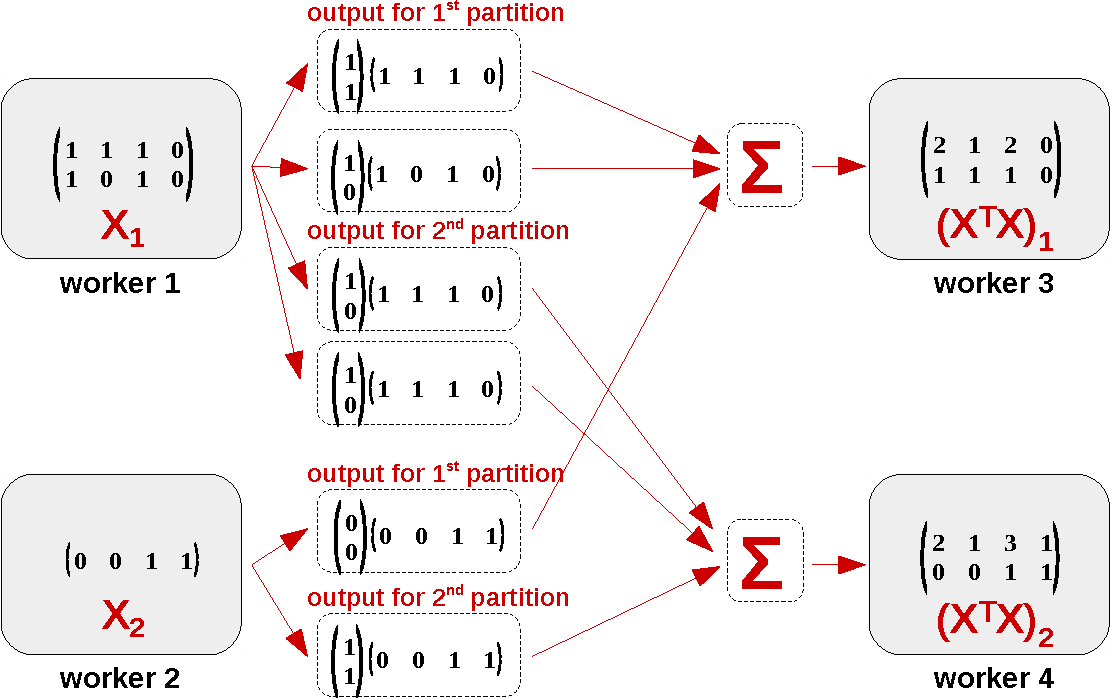
\includegraphics[scale=.35]{figures/ata-nonlocal-crop}
  \caption{Distributed computation of $X^{T}X$ via summation of partial outer products of rows.}
  \label{fig:atanonlocal}
        \end{subfigure}
  \hfill
         \begin{subfigure}[b]{0.45\textwidth}
  \centering
  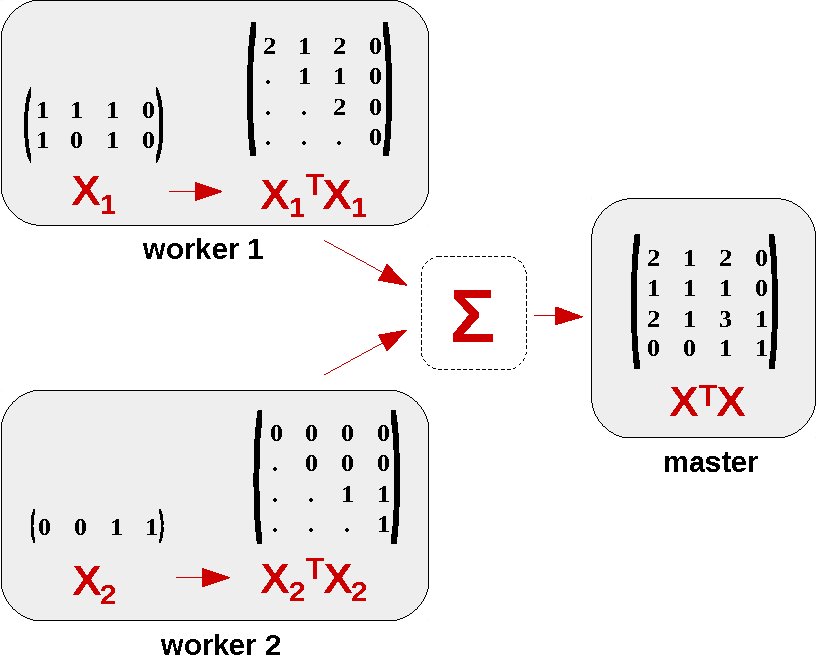
\includegraphics[scale=.35]{figures/ata-local-crop}
  \caption{Distributed computation of $X^{T}X$ via summation of partial outer products of rows.}
  \label{fig:atalocal}
        \end{subfigure}

        \caption{\label{fig:ataphysical} Physical execution strategies for computing a gram matrix.}
\end{figure}

\section{Limitations}

 - lack of native speed for in-core matrix operations, currently Colt, in the process of integrating ViennaCL~\cite{Tillet2013}
 - high variance in backed performance, e.g. lack of intermediate result caching in Flink

\section{Related Work}

{\em SystemML} \cite{Ghoting2011} - lightweight DSL instead of custom language (easier integration of external code), user decides on placement of matrices (e.g. in-core or in cluster), greatly simplifies the optimization. However, only non-holistic, non-cost-based optimization possible in Samsara, in contrast to~\cite{Boehm2014}

{\em SparkR} https://spark.apache.org/docs/latest/sparkr.html

{\em MLI} \cite{Sparks2013}

\section{Experimental Evaluation}

TODO: Show benefits of optimization

\section{Conclusion and Future Work}

% \section{Citations, figures, tables, references}
% \label{others}

% These instructions apply to everyone.

% \subsection{Citations within the text}

% The \verb+natbib+ package will be loaded for you by default.
% Citations may be author/year or numeric, as long as you maintain
% internal consistency.  As to the format of the references themselves,
% any style is acceptable as long as it is used consistently.

% The documentation for \verb+natbib+ may be found at
% \begin{center}
%   \url{http://mirrors.ctan.org/macros/latex/contrib/natbib/natnotes.pdf}
% \end{center}
% Of note is the command \verb+\citet+, which produces citations
% appropriate for use in inline text.  For example,
% \begin{verbatim}
%    \citet{hasselmo} investigated\dots
% \end{verbatim}
% produces
% \begin{quote}
%   Hasselmo, et al.\ (1995) investigated\dots
% \end{quote}

% If you wish to load the \verb+natbib+ package with options, you may
% add the following before loading the \verb+nips_2016+ package:
% \begin{verbatim}
%    \PassOptionsToPackage{options}{natbib}
% \end{verbatim}

% If \verb+natbib+ clashes with another package you load, you can add
% the optional argument \verb+nonatbib+ when loading the style file:
% \begin{verbatim}
%    \usepackage[nonatbib]{nips_2016}
% \end{verbatim}





% \subsection{Tables}

% All tables must be centered, neat, clean and legible.  The table
% number and title always appear before the table.  See
% Table~\ref{sample-table}.

% Place one line space before the table title, one line space after the
% table title, and one line space after the table. The table title must
% be lower case (except for first word and proper nouns); tables are
% numbered consecutively.

% Note that publication-quality tables \emph{do not contain vertical
%   rules.} We strongly suggest the use of the \verb+booktabs+ package,
% which allows for typesetting high-quality, professional tables:
% \begin{center}
%   \url{https://www.ctan.org/pkg/booktabs}
% \end{center}
% This package was used to typeset Table~\ref{sample-table}.

% \begin{table}[t]
%   \caption{Sample table title}
%   \label{sample-table}
%   \centering
%   \begin{tabular}{lll}
%     \toprule
%     \multicolumn{2}{c}{Part}                   \\
%     \cmidrule{1-2}
%     Name     & Description     & Size ($\mu$m) \\
%     \midrule
%     Dendrite & Input terminal  & $\sim$100     \\
%     Axon     & Output terminal & $\sim$10      \\
%     Soma     & Cell body       & up to $10^6$  \\
%     \bottomrule
%   \end{tabular}
% \end{table}

\newpage

{\small
  \bibliography{samsara}
  \bibliographystyle{plain}}

\end{document}
